{\LARGE Nozzle:}
The basic principal of nozzle is to accelerate the flow along its path. This
can be done with providing a special shape and pressure difference across the
inlet and outlet of the nozzle. For specific type of the flow the shape of nozzle
varies. This variation is as follows:
\begin{figure}[!h]
    \centering
    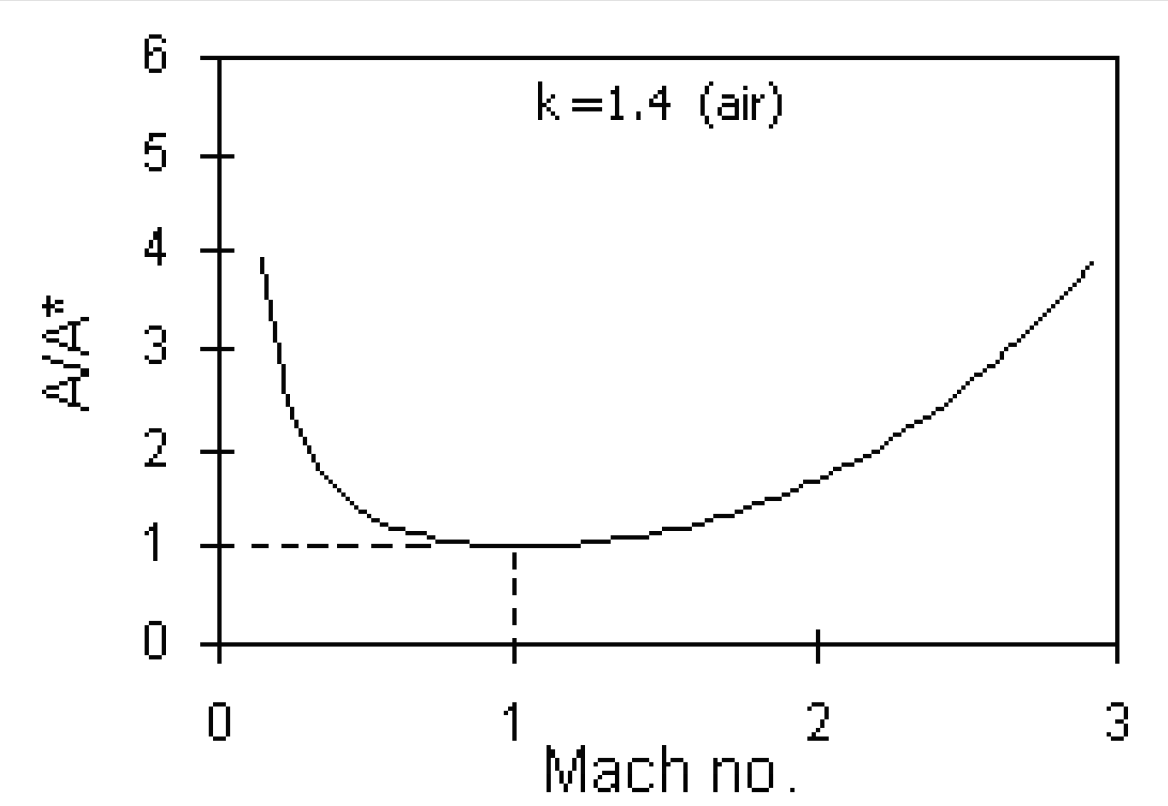
\includegraphics[width=8cm]{areaRatio.png}
    \caption{Area ratio variation with Mach number}
\end{figure}
\newline
Thus, for subsonic flow inlet convergent passage accelerates the flow and for
supersonic flow inlet divergent passage accelerates the flow. As we are going to
encounter flow from static chamber it is necessarily a subsonic flow at inlet.
\newline
Hence we are concerned with following two types of nozzle:
\begin{itemize}
    \item Convergent nozzle
    \item Convergent Divergent nozzle
\end{itemize}
\newpage

{\Large Convergent nozzle:}
This nozzle is mainly used to accelerate the flows till Mach number 1. The pressure distribution along the nozzle for various back pressure values are
shown in following graph.
\begin{figure}[!h]
    \centering
    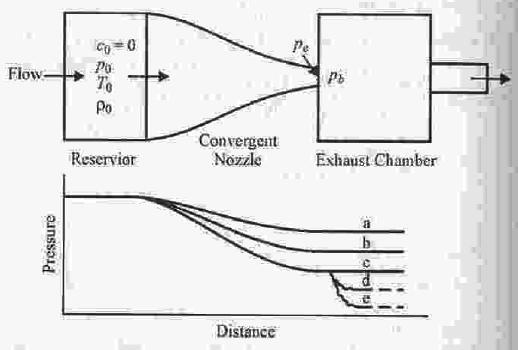
\includegraphics[width=8cm]{convergentNozzle.jpg}
    \caption{Pressure variation across convergent nozzle in Isentropic flow
conditions.}
\end{figure}
\newline
In curve 'a' and 'b', Pb is more than P* and hence, flow is accelerated at less than M=1. Curve 'c' represents design condition where flow is expanded to sonic conditions and Pb=P*. At curve 'c', maximum mass flow condition occurs. For curve 'd' and 'e', Pb<P* and discontinuity in the form of expansion wave occurs at outlet as nozzle can’t accelerate flow to achieve Pb . Thus, nozzle is said chocked at curve 'c' and mass flow rate is constant after that point. The mass flow parameter variation with back pressure variation is as shown below.
\begin{figure}[!h]
    \centering
    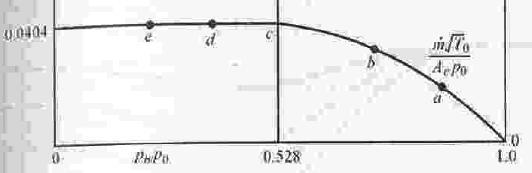
\includegraphics[width=8cm]{convergentMassFlow.jpg}
    \caption{Mass flow parameter variation with pressure ratio}
\end{figure}
\newpage

{\Large Convergent Divergent nozzle:}
This type of nozzle is used to accelerate the subsonic flows to the supersonic
conditions. This contains a convergent section which accelerates the flow to the
sonic condition to throat and a divergent section afterwards which accelerates the sonic flow to the supersonic conditions. Pressure distribution along its path for various back pressure conditions is as shown below.
\begin{figure}[!h]
    \centering
    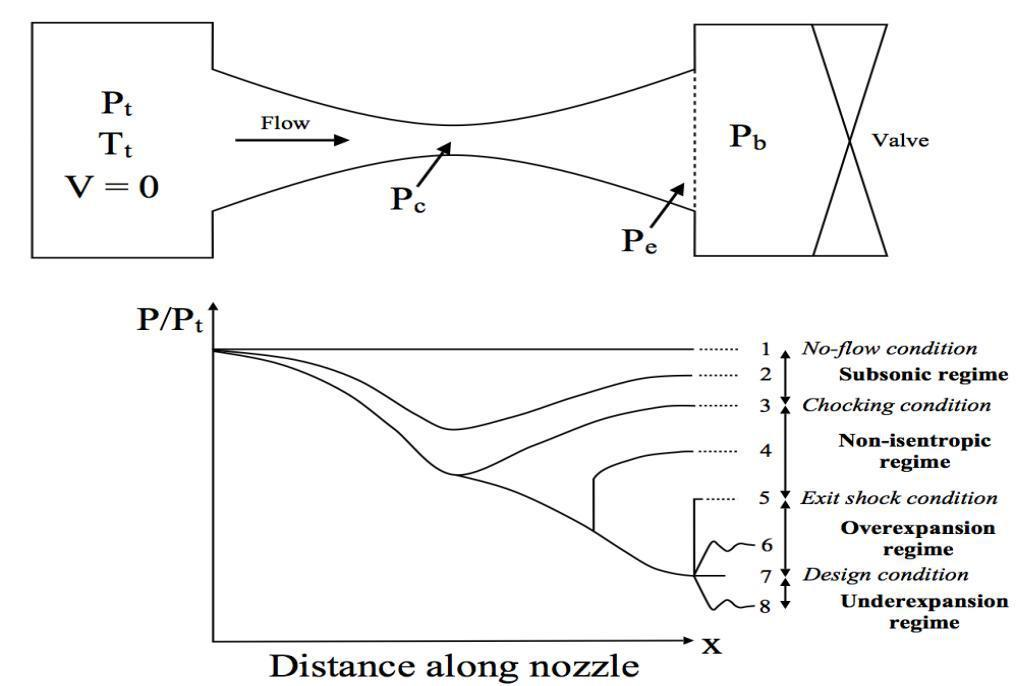
\includegraphics[width=7cm]{CD pressure distribution.jpg}
    \caption{Pressure distribution across CD nozzle}
\end{figure}
\newline
The Mach at throat is less than 1. Here divergent section behaves as diffuser
and increases the flow pressure to achieve Pb. Curve c shows choking condition at
throat i.e. M=1 and divergent section still acts a diffuser.
\newline
Further reducing Pb
means that the divergent section starts acting as nozzle. After some distance a
shock wave appears to increase the pressure and decrease the speed to subsonic.
This discontinuity occurs to match flow pressure to Pb. 
\newline
Curve 7 represents design
condition where expansion occurs in whole nozzle and no discontinuity forms.
This represents the maximum possible isentropic expansion done with nozzle.
\newline
Curve 8 represents the under expansion condition where exit pressure is more
than Pb. Thus, an expansion wave occurs at the exit of the nozzle.
Maximum mass flow parameter occurs at curve 3 and remains constant since. This represents the choking condition.
\newpage
All these mass flow variations can be seen in figure given below.
\begin{figure}[!h]
    \centering
    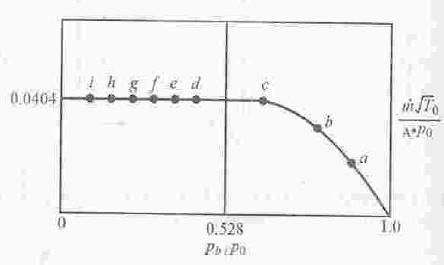
\includegraphics[width=6cm]{CD mass flow.jpg}
    \caption{Variation of mass flow parameter with pressure ratio}
\end{figure}
